\documentclass{standalone}
\usepackage{tikz}
%\usetikzlibrary{...}
\begin{document}
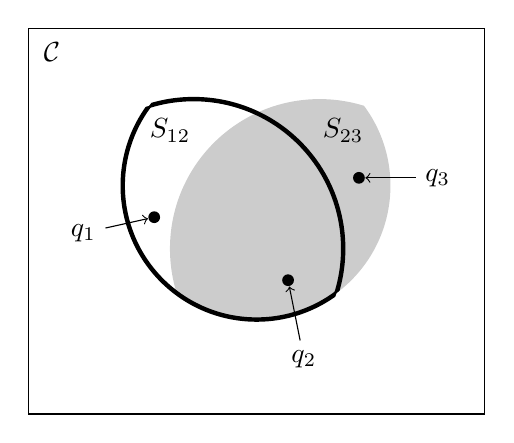
\begin{tikzpicture}

\draw (0,0) rectangle (5.8,4.9);

\coordinate (x) at (2.9,2.9);
\coordinate (y) at (2.1,2.1);
\coordinate (z) at (3.7,2.1);

\def\circlex{(x) circle (1.7)}
\def\circley{(y) circle (1.9)}
\def\circlez{(z) circle (1.9)}

% XnZ
\begin{scope}
   \clip \circlex;
   \fill[color=black!20] \circlez;
\end{scope}

% XnY
\begin{scope}
   \clip \circlex;
   %\fill[pattern=horizontal lines] \circley;
   \draw[ultra thick] \circley;
\end{scope}
\begin{scope}
   \clip \circley;
   \draw[ultra thick] \circlex;
\end{scope}

\node (clab) at (0.3,4.6) {$\mathcal{C}$};
\node[fill=white,circle,inner sep=0] (f1lab) at (1.8,3.6) {$S_{12}$};
\node (f2lab) at (4.0,3.6) {$S_{23}$};

\node[circle,fill=black,inner sep=1.5] (p1) at (1.6,2.5) {};
\node[circle,fill=black,inner sep=1.5] (p2) at (3.3,1.7) {};
\node[circle,fill=black,inner sep=1.5] (p3) at (4.2,3) {};

\node (p1lab) at (0.7,2.3) {$q_1$};
\node (p2lab) at (3.5,0.7) {$q_2$};
\node (p3lab) at (5.2,3.0) {$q_3$};
\draw[->] (p1lab) -- (p1);
\draw[->] (p2lab) -- (p2);
\draw[->] (p3lab) -- (p3);

\end{tikzpicture}%
\end{document}
